\documentclass[10pt, aspectratio=169]{beamer} %
\usetheme{Singapore}

\usepackage{bookmark}
\usepackage{graphicx}
\usepackage[english]{babel}
\usepackage[utf8]{inputenc}
\usepackage[T1]{fontenc}
\usepackage{amsmath}
\usepackage{color}
\usepackage{listings}
\usepackage{tabularx}
\usepackage{amssymb}
\usepackage{lmodern}

\usepackage{hyperref}
\hypersetup{colorlinks=true, urlcolor=blue}

\DeclareMathOperator*{\minimize}{minimize} %in preamble
 
\newcommand{\N}{{\mathbb{N}}}
\newcommand{\I}{{\bf I}}
\newcommand{\C}{{\bf C}}
\newcommand{\A}{{\bf A}}
\newcommand{\T}{{\bf T}}
\newcommand{\g}{{\bf g}}
\newcommand{\e}{{\bf e}}
\newcommand{\ab}{{\bf a}}
\newcommand{\ba}{{\bf b}}
\newcommand{\Z}{{\mathbb{Z}}}
\newcommand{\R}{{\mathbb{R}}}
\newcommand{\mbf}{\mathbf}
\newcommand{\bs}{\boldsymbol}
\newcommand{\cc}{{\bf c}}
\newcommand{\su}{{\sum_{n=0}^{N-1}}}

\newcommand{\argmax}{\mathop{\text{arg\;max}}}
\newcommand{\argmin}{\mathop{\text{arg\;min}}}

\newcommand{\HH}{{\bf H}}
\newcommand{\thb}{\boldsymbol{\theta}}
\newcommand{\w}{{\bf w}}
\newcommand{\Sigb}{\boldsymbol{\Sigma}}
\newcommand{\mub}{\boldsymbol{\mu}}
\newcommand{\alb}{\boldsymbol{\alpha}}

\newcommand{\s}{{\bf s}}
\newcommand{\SB}{{\bf S}}

\definecolor{blue}{RGB}{32,32,255}
\graphicspath{{./images/}}

\newcommand{\h}{{\bf h}}
\newcommand{\rr}{{\bf r}}
\newcommand{\X}{{\bf X}}
\newcommand{\x}{{\bf x}}
\newcommand{\y}{{\bf y}}
\newcommand{\p}{{\bf p}}
\newcommand{\E}{{\bf E}}
\newcommand{\U}{{\bf U}}
\newcommand{\V}{{\bf V}}
\newcommand{\f}{{\bf f}}
\newcommand{\var}{{\mathop{\text{var}}}}

\newcommand{\F}{{\cal F}}
\newcommand{\leveys}{0.75\textwidth}
\newcommand{\etaisyys}{0.25\textwidth}

\newcommand{\sinc}{\mathop{\text{sinc}}}
\newcommand{\esim}{\em}

\newcommand{\modulo}{\operatorname{mod}}

\setbeamertemplate{frametitle continuation}[from second] 

\renewcommand{\insertcontinuationtext}{}

\setbeamertemplate{frametitle}
{
	\vspace*{0.7cm} \vbox{\insertframetitle}
}

\usecolortheme{default}

\setbeamertemplate{mini frames}{}
\renewcommand*{\slideentry}[6]{}
\setbeamertemplate{frametitle}{
    \vspace*{0.2cm}
    \insertframetitle
}

\title{Pattern Recognition and Machine Learning}
\subtitle{Slide Set 6: Neural Networks and Deep Learning}
\author{Heikki Huttunen\\
heikki.huttunen@tut.fi}
\institute{Department of Signal Processing\\Tampere University of Technology}
\date{February 2017}

\begin{document}

\maketitle

\lstdefinestyle{mystyle}{
  belowcaptionskip=1\baselineskip,
  breaklines=true,
  frame=single,
  xleftmargin=\parindent,
  language=Python,
  showstringspaces=false,
  basicstyle=\tiny\ttfamily,
  keywordstyle=\bfseries\color{green!40!black},
  commentstyle=\itshape\color{purple!40!black},
  identifierstyle=\color{blue},
  stringstyle=\color{orange},
  moredelim=**[is][\color{red}]{@}{@},
}

\lstset{language=Python,style=mystyle} 



\begin{frame}{Traditional Neural Networks}
	
	\begin{itemize}
		\item Neural networks have been studied for decades.
		\item Traditional networks were \emph{fully connected} (also called \emph{dense}) networks consisting of typically 1-3 layers.
		\item Input dimensions were typically in the order of few hundred from a few dozen categories.
		\item Today, input may be 10k...100k variables from 1000 classes and network may have over 1000 layers.
	\end{itemize}
	\centering
	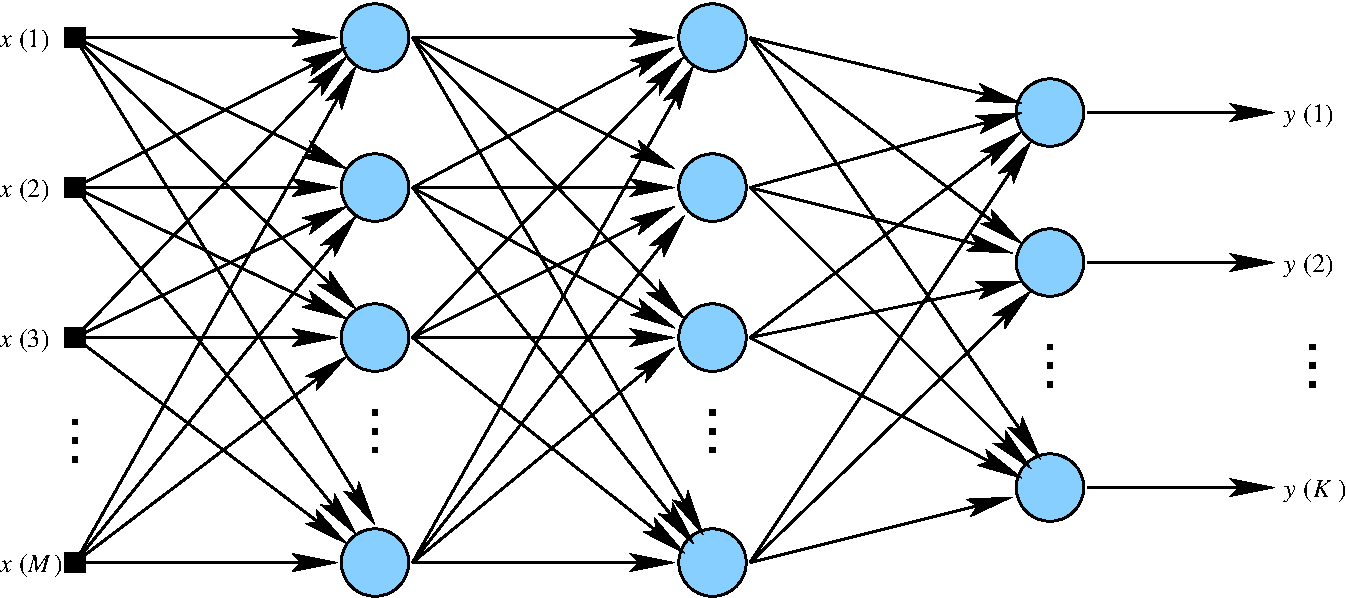
\includegraphics[width=0.6\textwidth]{VanillaNeuralNet.pdf}

\end{frame}

\begin{frame}{Traditional Neural Networks}
	
	\begin{itemize}
		\item The neuron of a vanilla network is illustrated below.
		\item In essence, the neuron is a dot product between the inputs $\x = (1, x_1, \ldots, x_n)$ and weights
		$\w = (w_0, w_1, \ldots, w_n)$ followed by a nonlinearity, most often \emph{logsig} or \emph{tanh}.
	\end{itemize}
	\centering
	\begin{columns}[onlytextwidth]
	\column{0.6\textwidth}
	\centerline{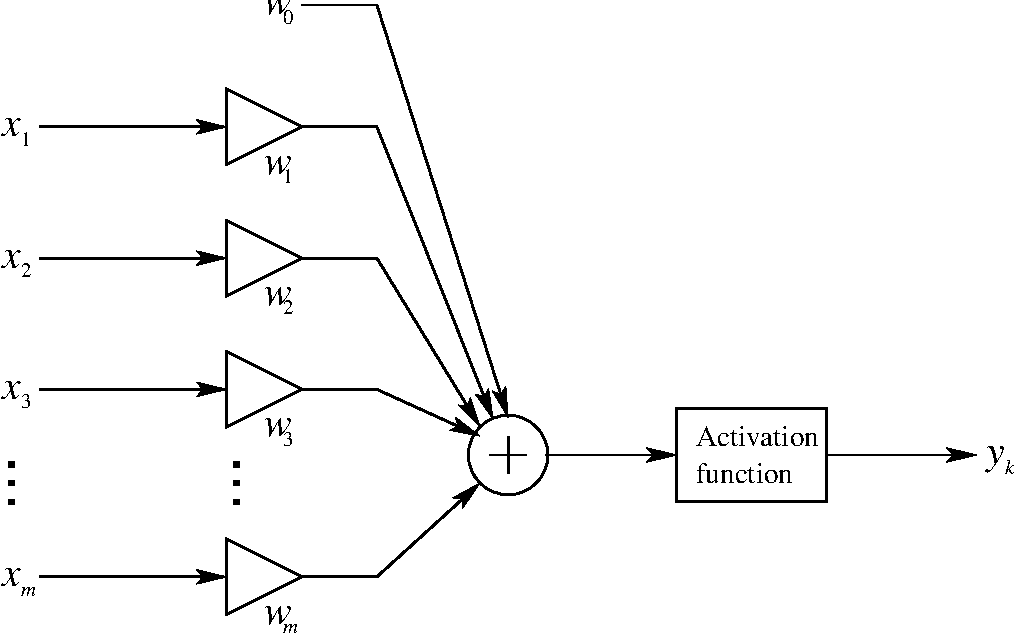
\includegraphics[width=0.75\textwidth]{Neuron.pdf}}
	\column{0.4\textwidth}
	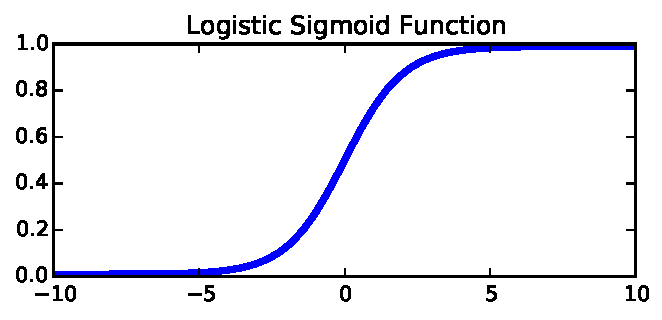
\includegraphics[width=0.8\textwidth]{sigmoid.pdf}\\
  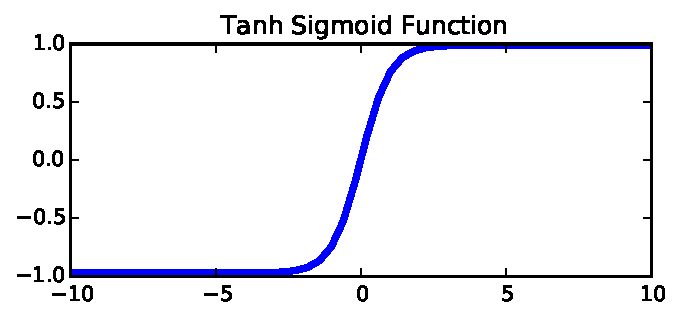
\includegraphics[width=0.8\textwidth]{sigmoid_tanh.pdf}
	\end{columns}
\begin{itemize}
	\item In other words: this is \emph{logistic regression} model, and 
	the full net is just a stack of logreg models.
\end{itemize}
\end{frame}

\begin{frame}{Training the Net}
	\begin{columns}
	\column{0.7\textwidth}
	\begin{itemize}
		\item Earlier, there was a lot of emphasis on training algorithms: \emph{conjugate gradient, Levenberg-Marquardt, etc.}
		\item Today, people mostly use \emph{stochastic gradient descent}.
	\end{itemize}
	\centerline{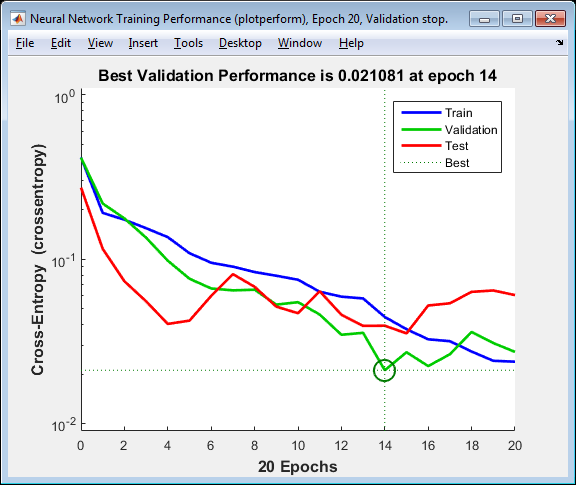
\includegraphics[width=0.5\textwidth]{nn_toolbox_training_error.png}}
\column{0.3\textwidth}
	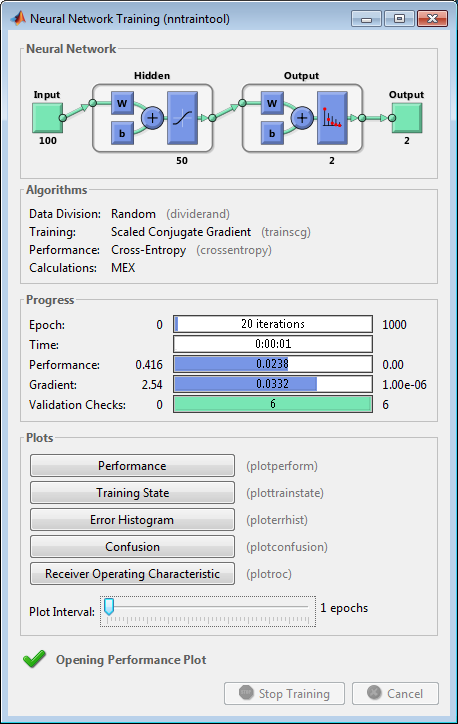
\includegraphics[width=\textwidth]{nn_toolbox.png}
	\end{columns}
\end{frame}


\begin{frame}{Backpropagation}
	\begin{columns}
	\column{0.7\textwidth}
	\begin{itemize}
		\item The network is trained by adjusting the weights according to the partial derivatives
		\[
		w_{ij} \leftarrow w_{ij} - \eta \frac{\partial {\cal E}}{\partial w_{ij}}
		\]

		\item In other words, the $j^\text{th}$ weight of the $i^\text{th}$ node 
		steps towards the negative gradient with step size $\eta > 0$.
		
		\item In the 1990's the network structure was rather fixed, and the formulae 
		would be derived by hand.
		
		\item Today, the same principle applies, but the exact form is computed symbolically.
		\end{itemize}
		
		\column{0.3\textwidth}
	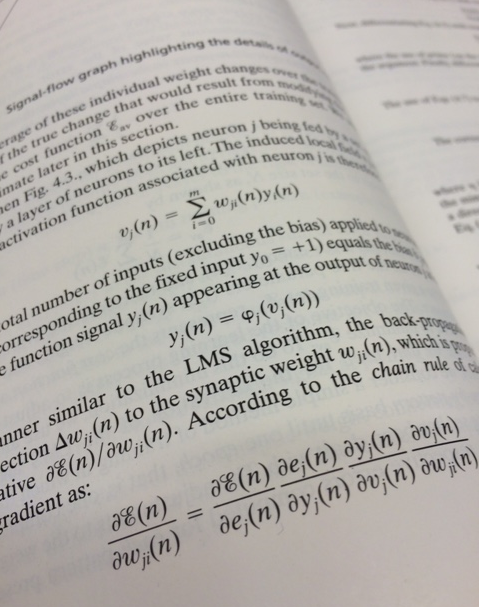
\includegraphics[width=\textwidth]{backpropagation.png}
	
	\emph{Backpropagation in Haykin: Neural networks, 1999.}
	\end{columns}
\end{frame}


\begin{frame}{Forward and Backward}
	\begin{itemize}
		\item Training has two passes: \emph{forward pass} and \emph{backward pass}.
		\item The forward pass feeds one (or more) samples to the net.
		\item The backward pass computes the (mean) error and propagates the gradients
		back adjusting the weights one at a time
		\item When all samples are shown to the net, one \emph{epoch} has passed. Typically the network
		runs for thousands of epochs.
		\end{itemize}
		
	\centerline{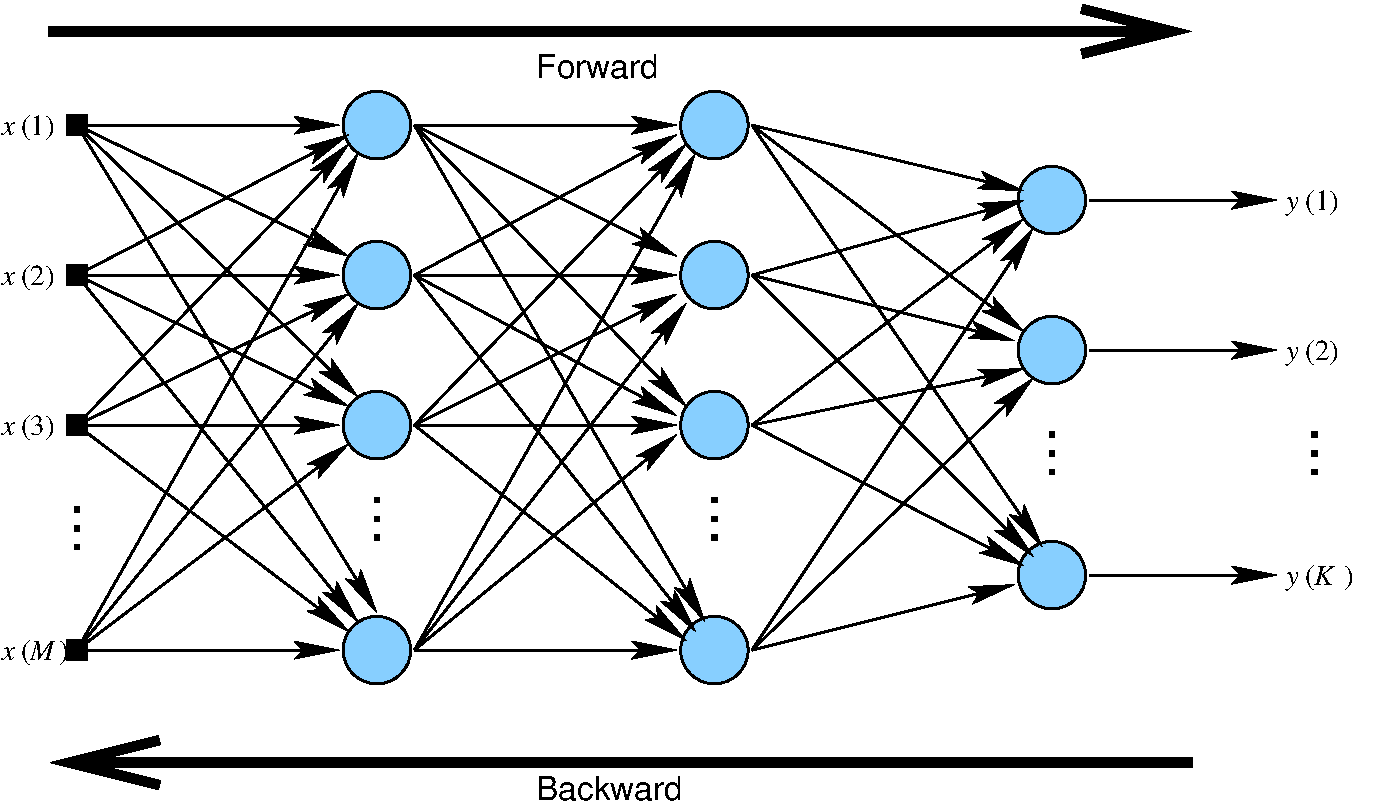
\includegraphics[width=0.5\textwidth]{VanillaNet_FB.pdf}}
	
\end{frame}


\begin{frame}{Neural Network Software}
	\begin{itemize}
\item Several packages exist:
\begin{itemize}
\item \textbf{Matlab NN Toolbox}: Obsolete. 
	\item \textbf{Caffe}: C++ / CUDA with Python and Matlab interfaces
\item \textbf{Theano}: Python based CUDA engine; several front ends available: e.g., \textbf{Keras} and Lasagne.
\item \textbf{Torch}: Library implemented in Lua language (Facebook). Also pyTorch interface exists since Jan 2017.
\item \textbf{TensorFlow}: Google deep learning engine. Open sourced in Nov 2015. Supported by \textbf{Keras}, which will be the default interface.
\item Others: VELES (Samsung), Minerva,...
\item Most use Nvidia \textbf{cuDNN} middle layer.
\end{itemize}
\item The important ones:
\begin{itemize}
\item \textbf{Caffe} is very fast and default in image recognition. Good Python and Matlab interface.
\item \textbf{Torch} has a large user base and lot of momentum from Facebook.
\item \textbf{Keras} is very flexible and readable full-python interface to Theano and Tensorflow.	\textbf{This is our choice for this course.}
\item \url{http://keras.io/} and \url{https://github.com/fchollet/keras}
\end{itemize}
\end{itemize}
\end{frame}

\begin{frame}[fragile]{Current Trends}
\begin{itemize}
	\item Python has become the language of machine learning.
\end{itemize}
\centering
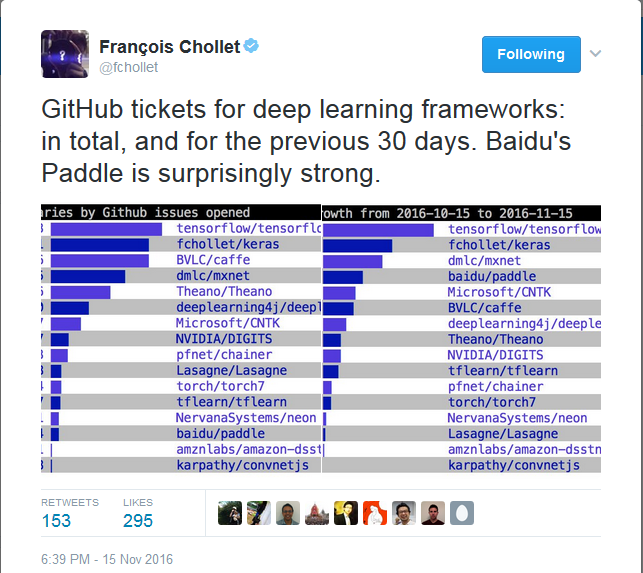
\includegraphics[width=0.3\textwidth]{images/dl-frameworks.png}\quad
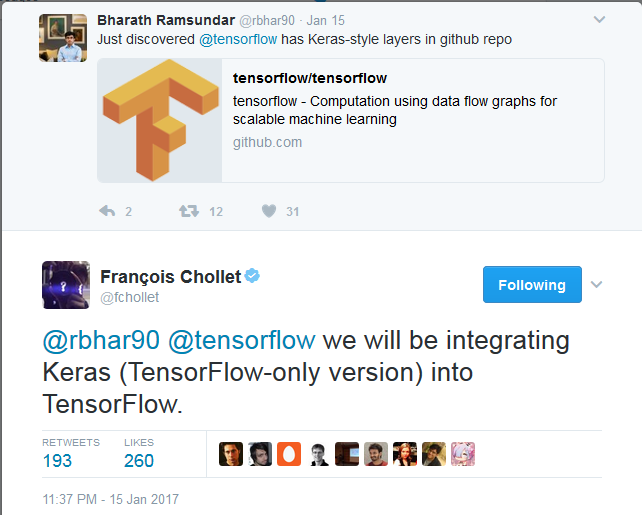
\includegraphics[width=0.3\textwidth]{images/keras-tf.png}\quad
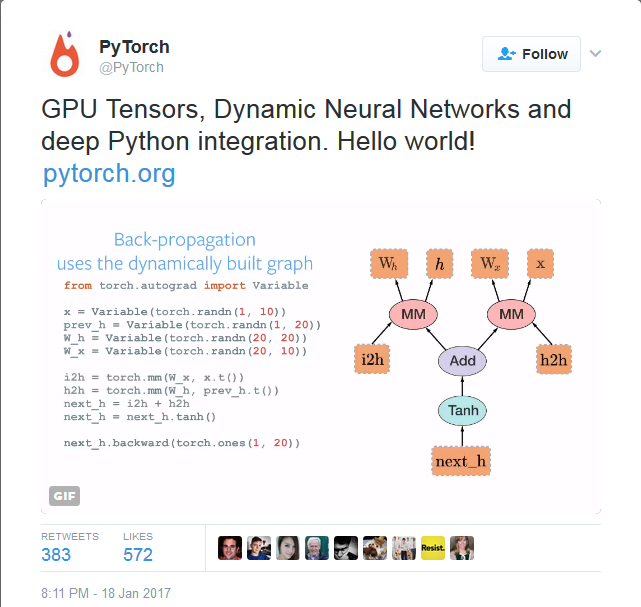
\includegraphics[width=0.3\textwidth]{images/pytorch.png}
\end{frame}

\begin{frame}[fragile]{Train a 2-layer Network with Keras}
\begin{columns}
\column{0.6\textwidth}
\begin{lstlisting}
# Training code:
from keras.models import Sequential
from keras.layers.core import Dense, Activation

# First we initialize the model. "Sequential" means there are no loops.
clf = Sequential()

# Add layers one at the time. Each with 100 nodes.
clf.add(Dense(100, input_dim=2, activation = 'sigmoid'))
clf.add(Dense(100, activation = 'sigmoid'))
clf.add(Dense(1, activation = 'sigmoid'))

# The code is compiled to CUDA or C++
clf.compile(loss='mean_squared_error', optimizer='sgd')
clf.fit(X, y, nb_epoch=20, batch_size=16) # takes a few seconds
\end{lstlisting}
\begin{lstlisting}
# Testing code:
# Probabilities
>>> clf.predict(np.array([[1, -2], [-3, -5]]))
array([[ 0.50781795],
       [ 0.48059484]])
# Classes
>>> clf.predict(np.array([[1, -2], [-3, -5]])) > 0.5
array([[ True],
       [False]], dtype=bool)
\end{lstlisting}
\column{0.3\textwidth}
\centerline{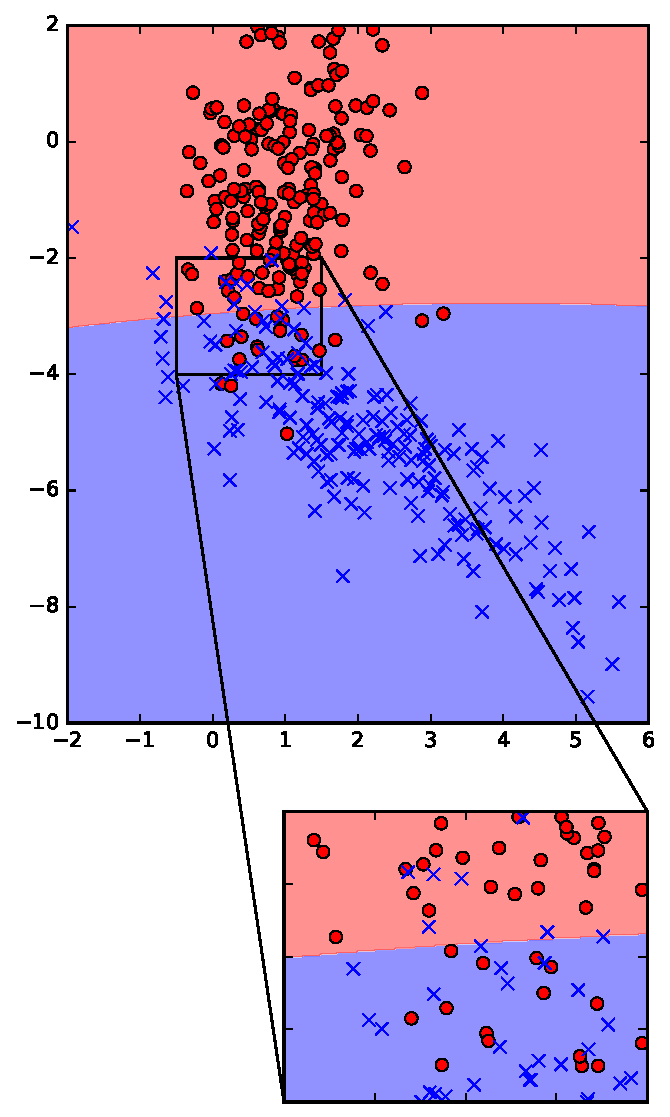
\includegraphics[width=\columnwidth]{mlp.pdf}}
\end{columns}
\end{frame}

\begin{frame}{Deep Learning}
	\begin{itemize}
		\item The neural network research was rather silent after the rapid expansion in the 1990's.
		\item The hot topic of 2000's were, \emph{e.g.,} the SVM and \emph{big data}.
		\item However, at the end of the decade, neural networks started to gain popularity again:
		A group at Univ. Toronto led by Prof. Geoffrey Hinton studied unconventionally \textbf{deep} networks
		using \emph{unsupervised} pretraining.
		\item He discovered that training of large networks was indeed possible with 
		an unsupervised pretraining step that initializes the network weights in a layerwise manner.
		\item Another key factor to the success was the rapidly increased computational power brought 
		by recent Graphics Processing Units (GPU's).
		\end{itemize}
\end{frame}

\begin{frame}{Unsupervised Pretraining}
	\begin{itemize}
		\item There were two key problems why network depth did not increase beyond 2-3 layers:
		\begin{enumerate}
			\item The error has huge \textbf{local minima areas} when the net becomes deep: Training gets stuck at one of them.
			\item The \textbf{gradient vanishes} at the bottom layers: The logistic activation function tends to decrease the gradient magnitude at each layer;
			eventually the gradient at the bottom layer is very small and they will not train at all.
		\end{enumerate}
		\item The former problem was corrected by \textbf{unsupervised} pretraining:
		\begin{itemize}
			\item Train
		layered models that learned to \emph{represent} the data (no class labels, no classification, just
		try to learn to reproduce the data).
		\item Initialize the network with the weights of the unsupervised model and train in a supervised setting.
		\item Common tools: \emph{restricted Boltzmann machine} (RBM), \emph{deep belief network} (DBN), 
		\emph{autoencoders}, etc.
		\end{itemize}
		\end{itemize}
\end{frame}


\begin{frame}[fragile,allowframebreaks=0.8]{Back to Supervised Training}
\begin{columns}[onlytextwidth]
\column{0.8\textwidth}
	\begin{itemize}
		\item After the excitement of deep networks was triggered, the study of fully
		supervised approaches started as well (purely supervised training is more familiar,
		well explored and less scary angle of approach).
		\item A few key discoveries avoid the need for pretraining:
		\begin{itemize}
			\item New activation functions that better preserve the gradient over layers; most importantly the
			Rectified Linear Unit\footnote{\tiny Glorot, Bordes, and Bengio. "Deep sparse rectifier neural networks."}: $\text{ReLU}(x) = \max(0, x)$.
			\item Novel weight initialization techniques; \emph{e.g.,} Glorot initialization (aka. Xavier initialization) adjusts the initial weight magnitudes layerwise\footnote{\tiny Glorot and Bengio. "Understanding the difficulty of training deep feedforward neural networks."}.
			\item Dropout regularization; avoid overfitting by injecting noise to the network\footnote{\tiny Srivastava, Hinton, Krizhevsky, Sutskever and Salakhutdinov. "Dropout: A simple way to prevent neural networks from overfitting."}. Individual neurons are shut down at random in the training phase.
		\end{itemize}
		\end{itemize}
\column{0.2\textwidth}
\hspace*{-2cm}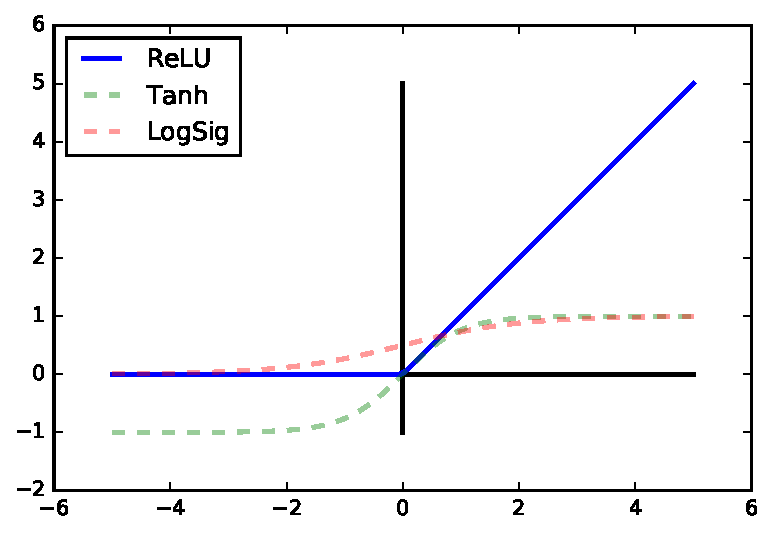
\includegraphics[width=\columnwidth]{images/ReLU.pdf}
\end{columns}
\end{frame}

\begin{frame}[fragile,allowframebreaks=0.8]{Convolutional Layers}

	\begin{itemize}
		\item In addition to the novel techniques for training, also new network architectures 
		have been adopted.
		\item Most important of them is \emph{convolutional layer}, which preserves also the topology
		of the input.
		\item Convolutional network was proposed already in 1989 but had a rather marginal role
		as long as image size was small (\emph{e.g.,} 1990's MNIST dataset of size $28\times 28$ as compared
		to current ImageNet benchmark of size $256\times 256$).
		\end{itemize}
\end{frame}

\begin{frame}[fragile]{Convolutional Network}

	\begin{itemize}
		\item 	The typical structure of a convolutional network repeats the following elements:
		
			 \fbox{\textbf{convolution}} $\Rightarrow$ \fbox{\textbf{ReLU}} $\Rightarrow$ \fbox{\textbf{subsampling}}
			
		\begin{enumerate}
	
	\item \textbf{Convolution} filters the input with a number of convolutional kernels. In the first layer these
	can be, \emph{e.g.,} $9\times 9\times 3$; \emph{i.e.,} they see the local window from all RGB layers.
	\begin{itemize}
		\item The results are called \textbf{feature maps}, and there are typically a few dozen of those.
	\end{itemize}
	\item \textbf{ReLU} passes the feature maps through a pixelwise ReLU. 
	\begin{itemize}
		\item In numpy: \verb+y = numpy.maximum(x, 0)+.
			\end{itemize}
	\item \textbf{Subsampling} shrinks the input dimensions by an integer factor.
	\begin{itemize}
		\item Originally this was done by averaging each $2\times 2$ block.
		\item Nowadays,
		\textbf{maxpooling} is more common (take max of each $2\times 2$ block).
		\item Subsampling reduces the data size and improves spatial invariance.
			\end{itemize}
		\end{enumerate}
	\end{itemize}
%	\centering
%	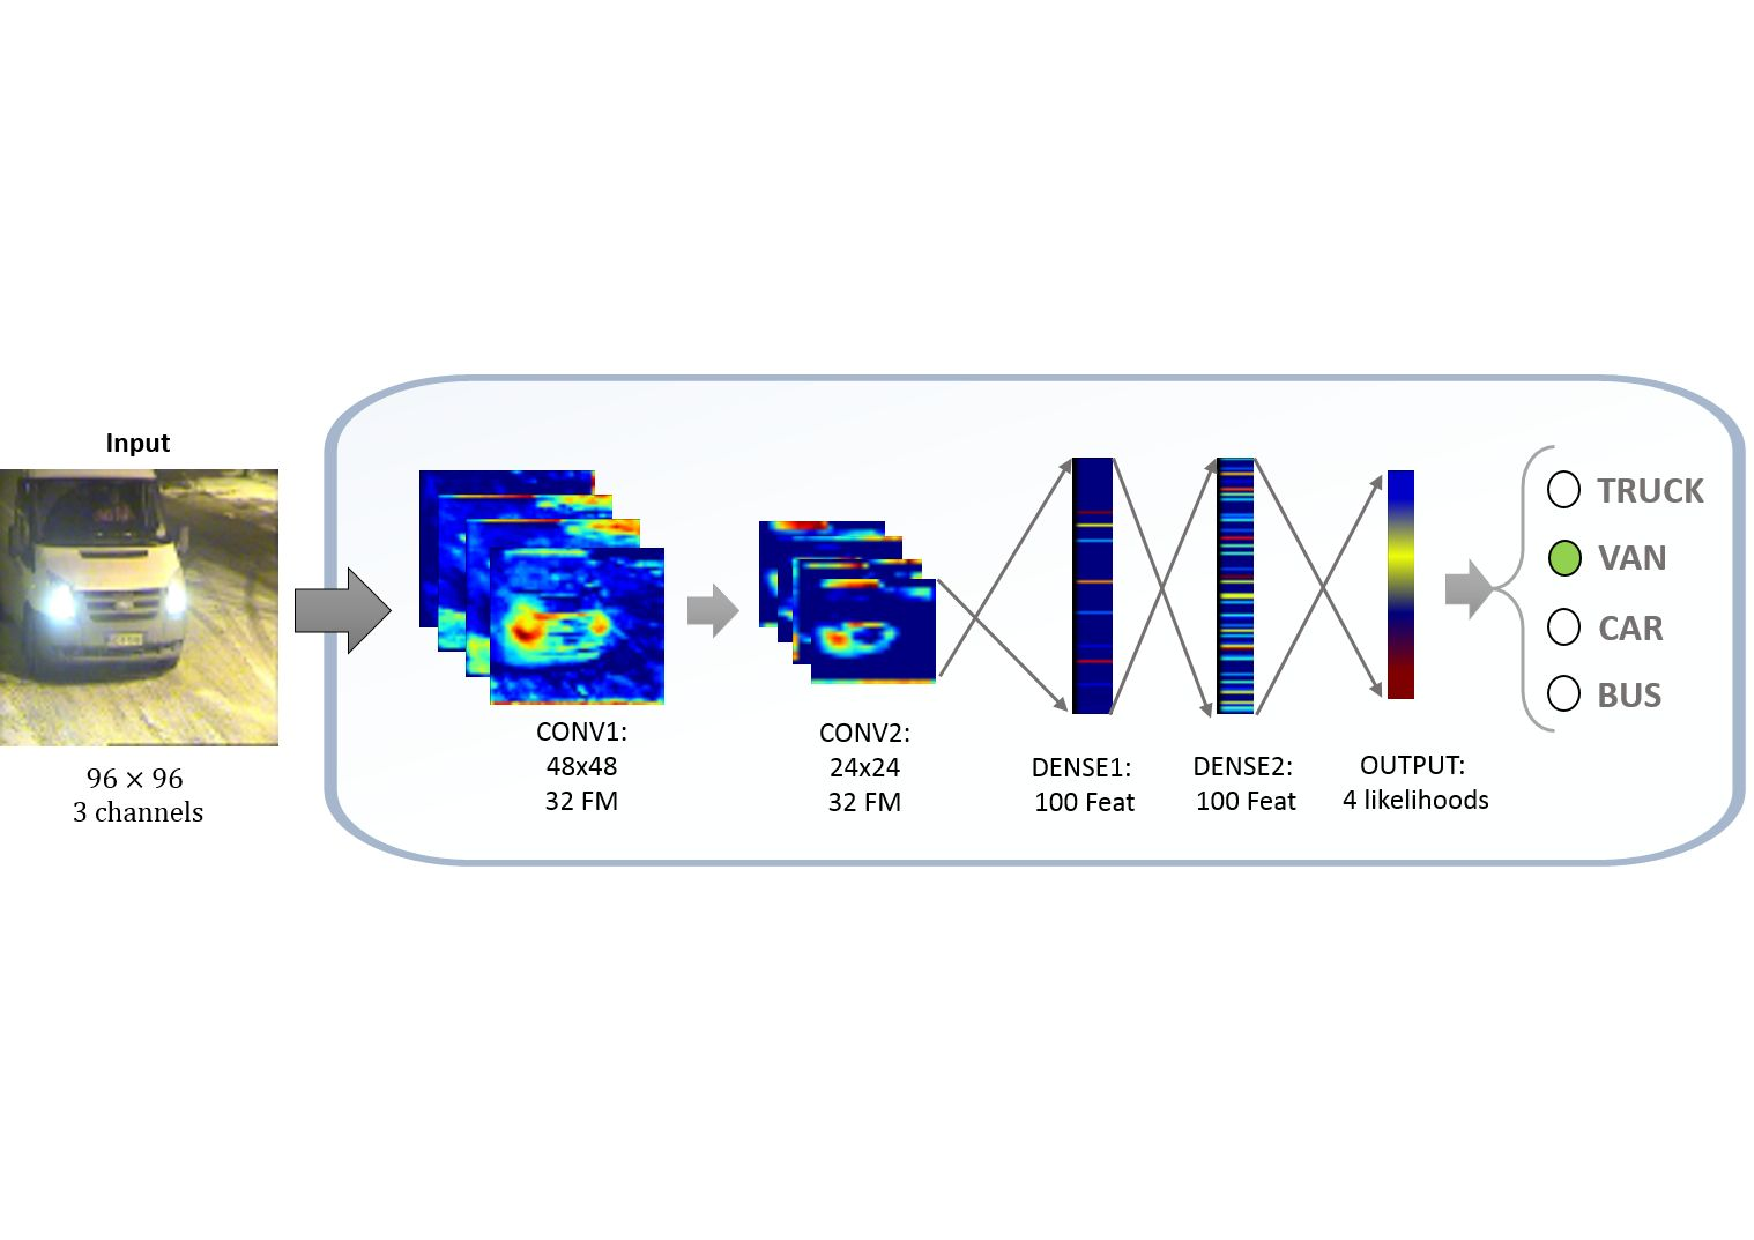
\includegraphics[width=0.8\textwidth]{ConvMaps.pdf}

\end{frame}


\begin{frame}{Convolutional Network}

\centerline{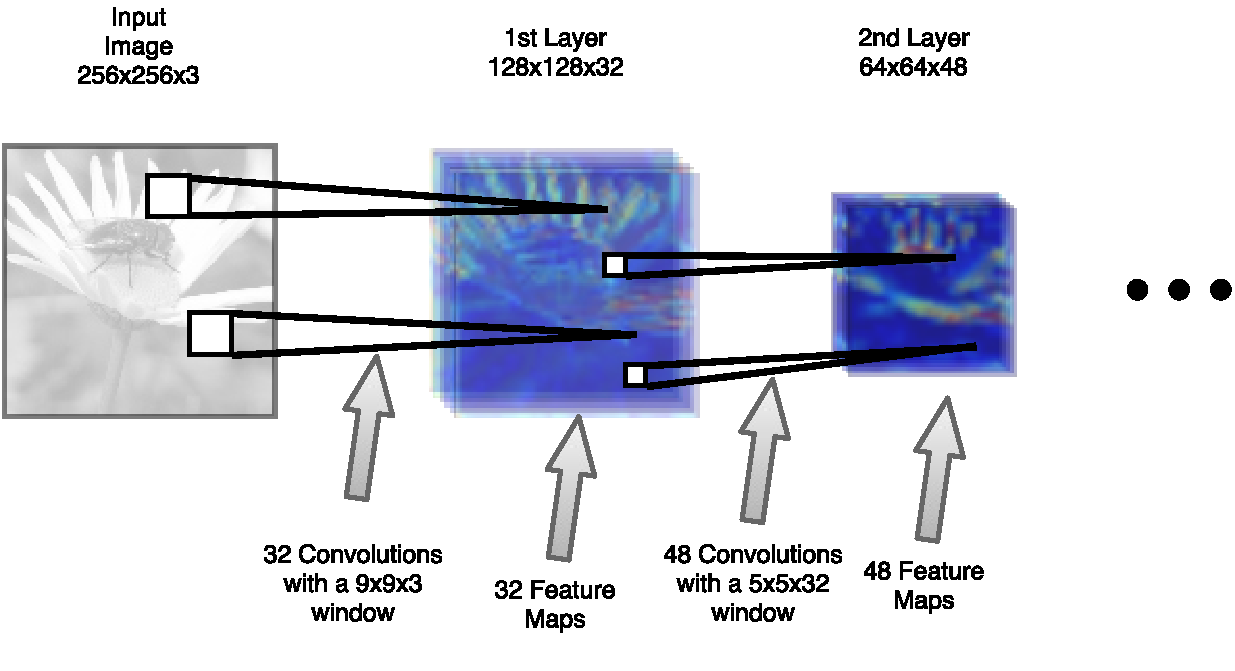
\includegraphics[width=0.8\textwidth]{ConvNet_karpanen.pdf}}

\end{frame}

\begin{frame}[fragile]{Convolutional Network: Example}
\begin{columns}
\column{0.75\textwidth}
\begin{itemize}
	\item Let's train a convnet with the famous MNIST dataset.
	\item MNIST consists of 60000 training and 10000 test images
	representing handwritten numbers from US mail.
	\item Each image is $28\times 28$ pixels and there are 10 categories.
	\item Generally considered an easy problem: Logistic regression
	gives over 90\% accuracy and convnet can reach (almost) 100\%.
	\item However, 10 years ago, the state of the art error was still over 1\%.
\end{itemize}
\column{0.2\textwidth}
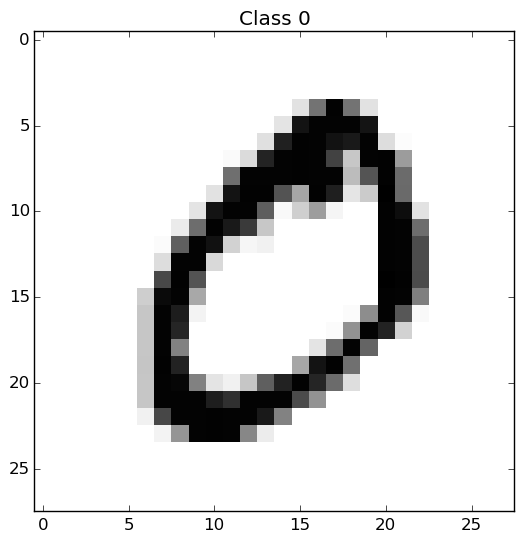
\includegraphics[width=0.45\textwidth]{mnist_0.png}
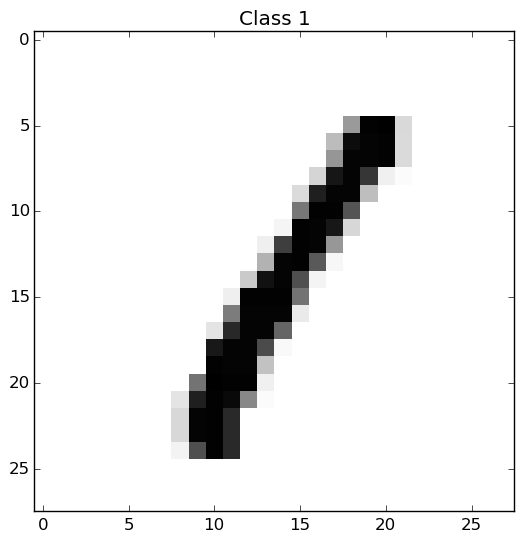
\includegraphics[width=0.45\textwidth]{mnist_1.png}\\
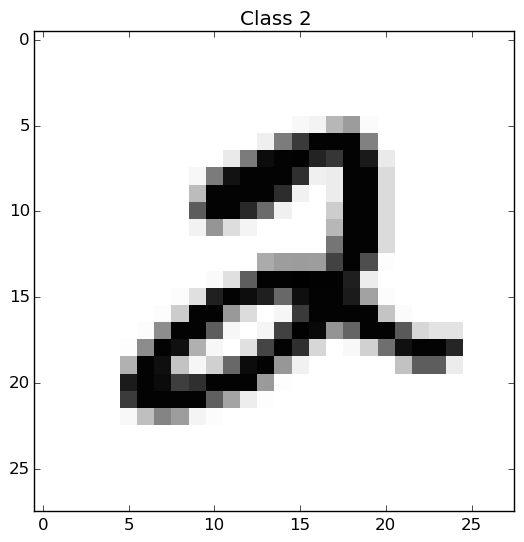
\includegraphics[width=0.45\textwidth]{mnist_2.png}
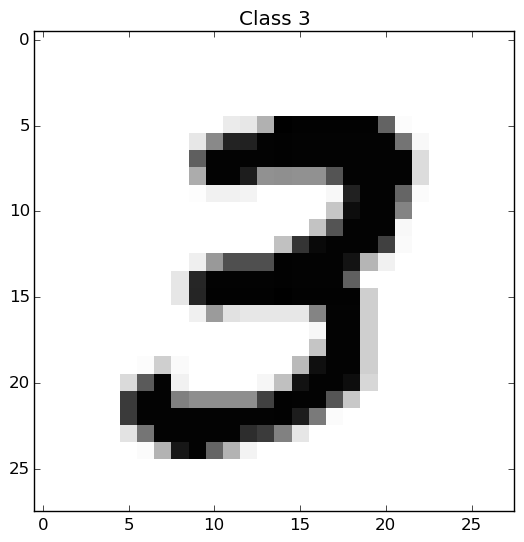
\includegraphics[width=0.45\textwidth]{mnist_3.png}\\
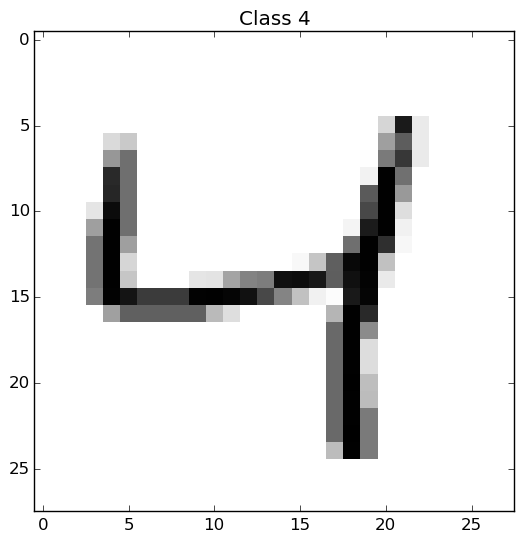
\includegraphics[width=0.45\textwidth]{mnist_4.png}
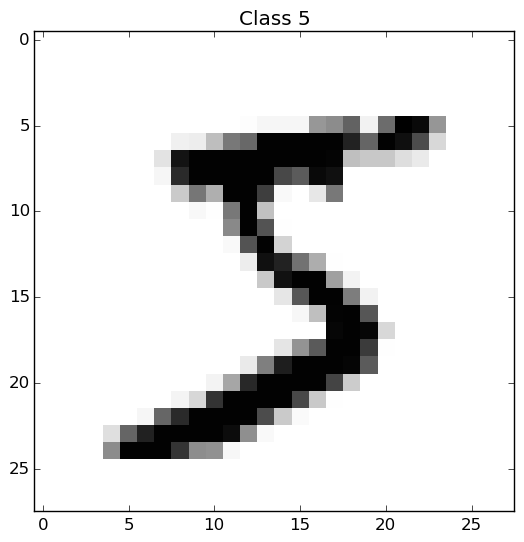
\includegraphics[width=0.45\textwidth]{mnist_5.png}\\
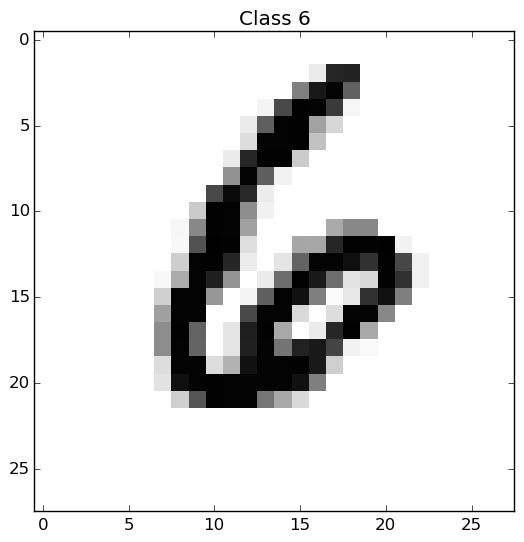
\includegraphics[width=0.45\textwidth]{mnist_6.png}
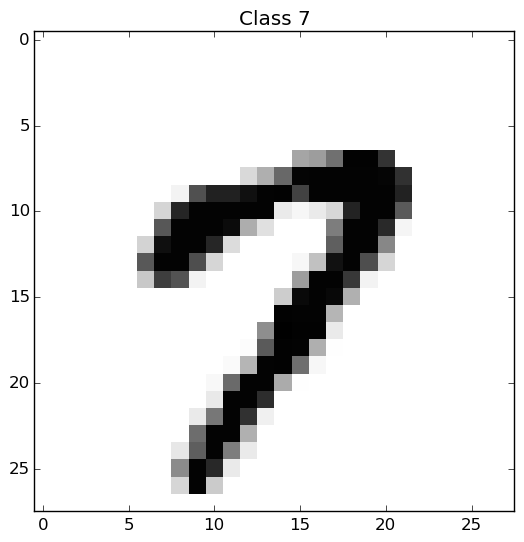
\includegraphics[width=0.45\textwidth]{mnist_7.png}\\
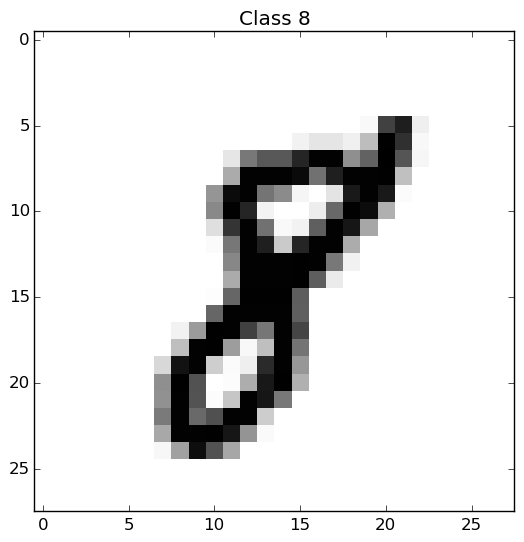
\includegraphics[width=0.45\textwidth]{mnist_8.png}
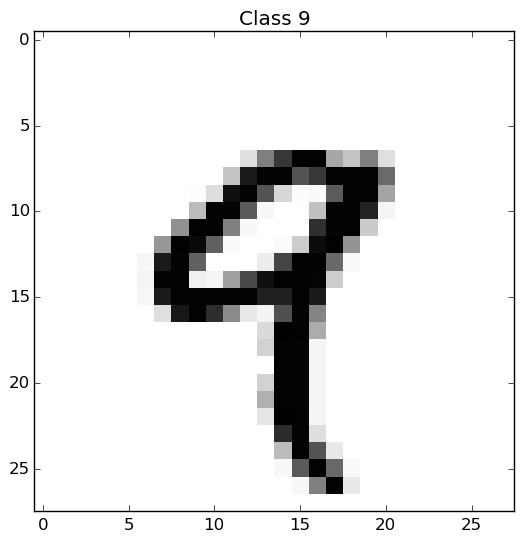
\includegraphics[width=0.45\textwidth]{mnist_9.png}
\end{columns}
\end{frame}


\begin{frame}[fragile]{Convolutional Network: Example}
\begin{columns}
\column{0.47\textwidth}
\begin{lstlisting}
# Training code (modified from mnist_cnn.py at Keras examples)
from keras.datasets import mnist
from keras.models import Sequential
from keras.layers.core import Dense, Dropout, Activation, Flatten
from keras.layers.convolutional import Convolution2D, MaxPooling2D

# We use the handwritten digit database "MNIST".
# 60000 training and 10000 test images of 
# size 28x28
(X_train, y_train), (X_test, y_test) = mnist.load_data()

num_featmaps = 32   # This many filters per layer
num_classes = 10    # Digits 0,1,...,9
num_epochs = 50     # Show all samples 50 times
w, h = 5, 5         # Conv window size
\end{lstlisting}

\column{0.53\textwidth}
\begin{lstlisting}
model = Sequential()

# Layer 1: needs input_shape as well.
model.add(Convolution2D(num_featmaps, w, h,
          input_shape=(1, 28, 28), 
          activation = 'relu'))

# Layer 2:
model.add(Convolution2D(num_featmaps, w, h, activation = 'relu'))
model.add(MaxPooling2D(pool_size=(2, 2)))
model.add(Dropout(0.25))

# Layer 3: dense layer with 128 nodes
# Flatten() vectorizes the data:
# 32x10x10 -> 3200 
# (10x10 instead of 14x14 due to border effect)
model.add(Flatten()) 
model.add(Dense(128, activation = 'relu'))
model.add(Dropout(0.5))

# Layer 4: Last layer producing 10 outputs.
model.add(Dense(num_classes, activation='softmax'))

# Compile and train
model.compile(loss='categorical_crossentropy', optimizer='adadelta')
model.fit(X_train, Y_train, nb_epoch=100)
\end{lstlisting}
\end{columns}
\end{frame}

\begin{frame}[fragile]{Convolutional Network: Training Log}
\begin{itemize}
	\item The code runs for about 5-10 minutes on a GPU.
	\item On a CPU, this would take 1-2 hours (1 epoch $\approx$ 500 s)
\end{itemize}
\begin{lstlisting}[
    basicstyle=\tiny, %or \small or \footnotesize etc.
]
Using gpu device 0: Tesla K40m 
Using Theano backend.
Compiling model...
Model compilation took 0.1 minutes.
Training...
Train on 60000 samples, validate on 10000 samples
Epoch 1/10
60000/60000 [================] - 31s - loss: 0.2193 - acc: 0.9322 - val_loss: 0.0519 - val_acc: 0.9835
Epoch 2/10
60000/60000 [================] - 31s - loss: 0.0807 - acc: 0.9758 - val_loss: 0.0398 - val_acc: 0.9863
Epoch 3/10
60000/60000 [================] - 31s - loss: 0.0581 - acc: 0.9825 - val_loss: 0.0322 - val_acc: 0.9898
Epoch 4/10
60000/60000 [================] - 31s - loss: 0.0500 - acc: 0.9851 - val_loss: 0.0276 - val_acc: 0.9913
Epoch 5/10
60000/60000 [================] - 31s - loss: 0.0430 - acc: 0.9872 - val_loss: 0.0287 - val_acc: 0.9906
Epoch 6/10
60000/60000 [================] - 31s - loss: 0.0387 - acc: 0.9882 - val_loss: 0.0246 - val_acc: 0.9922
Epoch 7/10
60000/60000 [================] - 31s - loss: 0.0352 - acc: 0.9897 - val_loss: 0.0270 - val_acc: 0.9913
Epoch 8/10
60000/60000 [================] - 31s - loss: 0.0324 - acc: 0.9902 - val_loss: 0.0223 - val_acc: 0.9928
Epoch 9/10
60000/60000 [================] - 31s - loss: 0.0294 - acc: 0.9907 - val_loss: 0.0221 - val_acc: 0.9926
Epoch 10/10
60000/60000 [================] - 31s - loss: 0.0252 - acc: 0.9922 - val_loss: 0.0271 - val_acc: 0.9916
Training (10 epochs) took 5.8 minutes.
\end{lstlisting}
\end{frame}

\begin{frame}[fragile]{Save and Load the Net}
\begin{itemize}
	\item The network can be saved and loaded to disk in a straightforward manner:
	\begin{itemize}
		\item \textbf{Saving:}
\begin{lstlisting}
model.save("my_net.h5")
\end{lstlisting}
		\item \textbf{Loading:} 
\begin{lstlisting}
from keras.models import load_model
load_model("my_net.h5")
\end{lstlisting}
\end{itemize}
\item Network is saved in HDF5 format.
HDF5 is a serialization format similar to \verb+.mat+ or \verb+.pkl+
although a lot more efficient.
\item Use HDF5 for data storage with \verb+h5py+.
\begin{lstlisting}
# Save np.array X to h5 file:
import h5py
with h5py.File("my_data.h5", "w") as h5:
   h5["X"] = X
\end{lstlisting}

\begin{lstlisting}
# Load np.array X from h5 file:
import h5py
with h5py.File("my_data.h5", "r") as h5:
   X = np.array(h5["X"])
	
# Note: Don't cast to numpy unless necessary.
# Data can be accessed from h5 directly.
\end{lstlisting}

\end{itemize}
\end{frame}


\begin{frame}[fragile]{Network Structure}
\begin{columns}
\column{0.75\textwidth}
\begin{itemize}
	\item It is possible to look into the filters on the convolutional layers.
\begin{lstlisting}
# First layer weights (shown on the right):
weights = model.layers[0].get_weights()[0]
\end{lstlisting}
\item The second layer is difficult to visualize, because the input is 32-dimensional:
\begin{lstlisting}
# Zeroth layer weights:
>>> model.layers[0].get_weights()[0].shape
(32, 1, 5, 5)
# First layer weights:
>>> model.layers[1].get_weights()[0].shape
(32, 32, 5, 5)
\end{lstlisting}
\item The dense layer is the 5th (conv $\rightarrow$ conv $\rightarrow$ maxpool $\rightarrow$ dropout $\rightarrow$ flatten $\rightarrow$ dense).
\begin{lstlisting}
# Fifth layer weights map 3200 inputs to 128 outputs.
# This is actually a matrix multiplication.
>>> model.layers[5].get_weights()[0].shape
(3200, 128) 
\end{lstlisting}
	\end{itemize}
\column{0.25\textwidth}
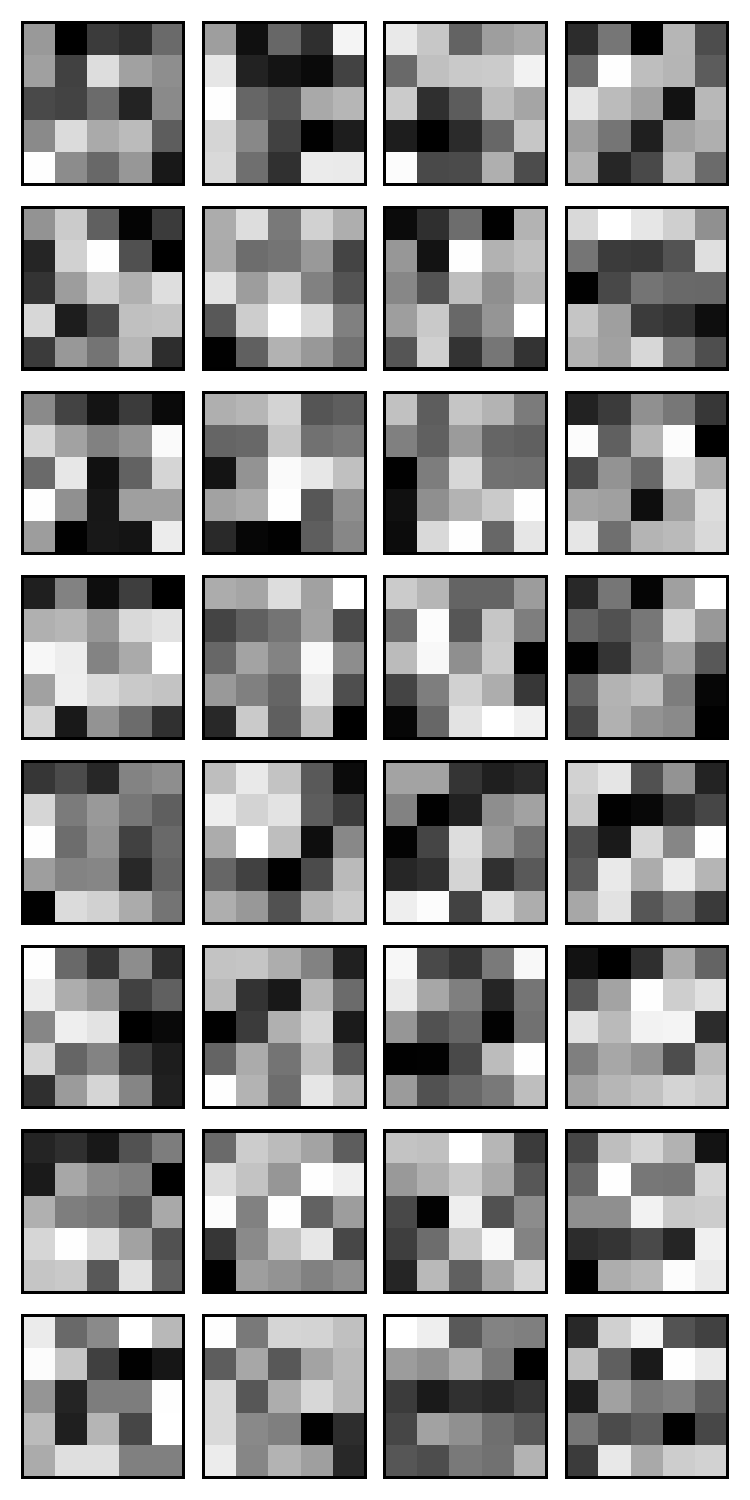
\includegraphics[width=\textwidth]{keras_l1_filters.pdf}
\end{columns}
\end{frame}



\begin{frame}[fragile]{Network Activations}
\begin{columns}
\column{0.6\textwidth}
\begin{itemize}
	\item The layer outputs are usually more interesting than the filters.
	\item These can be visualized as well.
	\item For details, see \href{http://keras.io/faq/#how-can-i-visualize-the-output-of-an-intermediate-layer}{Keras FAQ}.
	%\item Note: the outputs are actually grayscale; here in color only for better visualization.
	\end{itemize}
\column{0.2\textwidth}
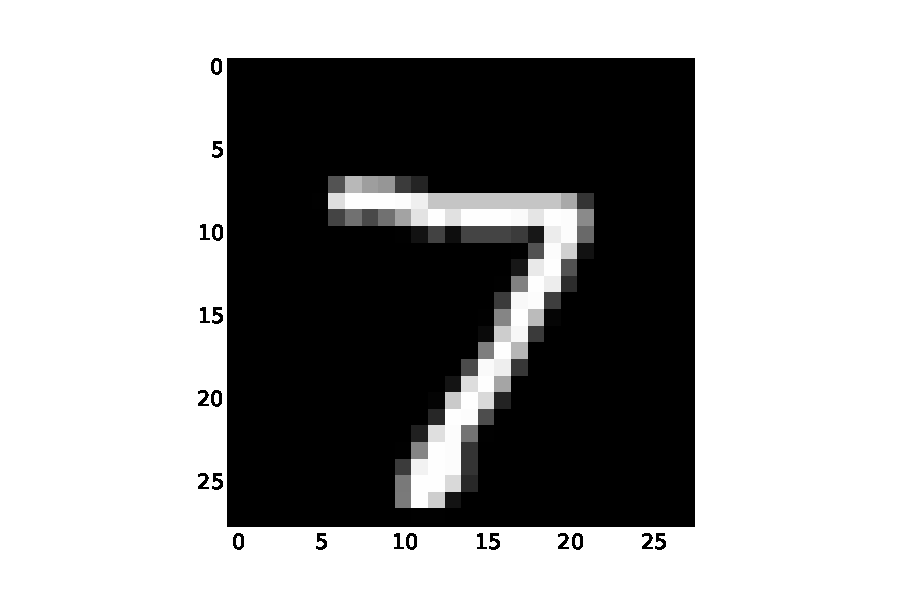
\includegraphics[width=\textwidth]{keras_l1_input.pdf}\\
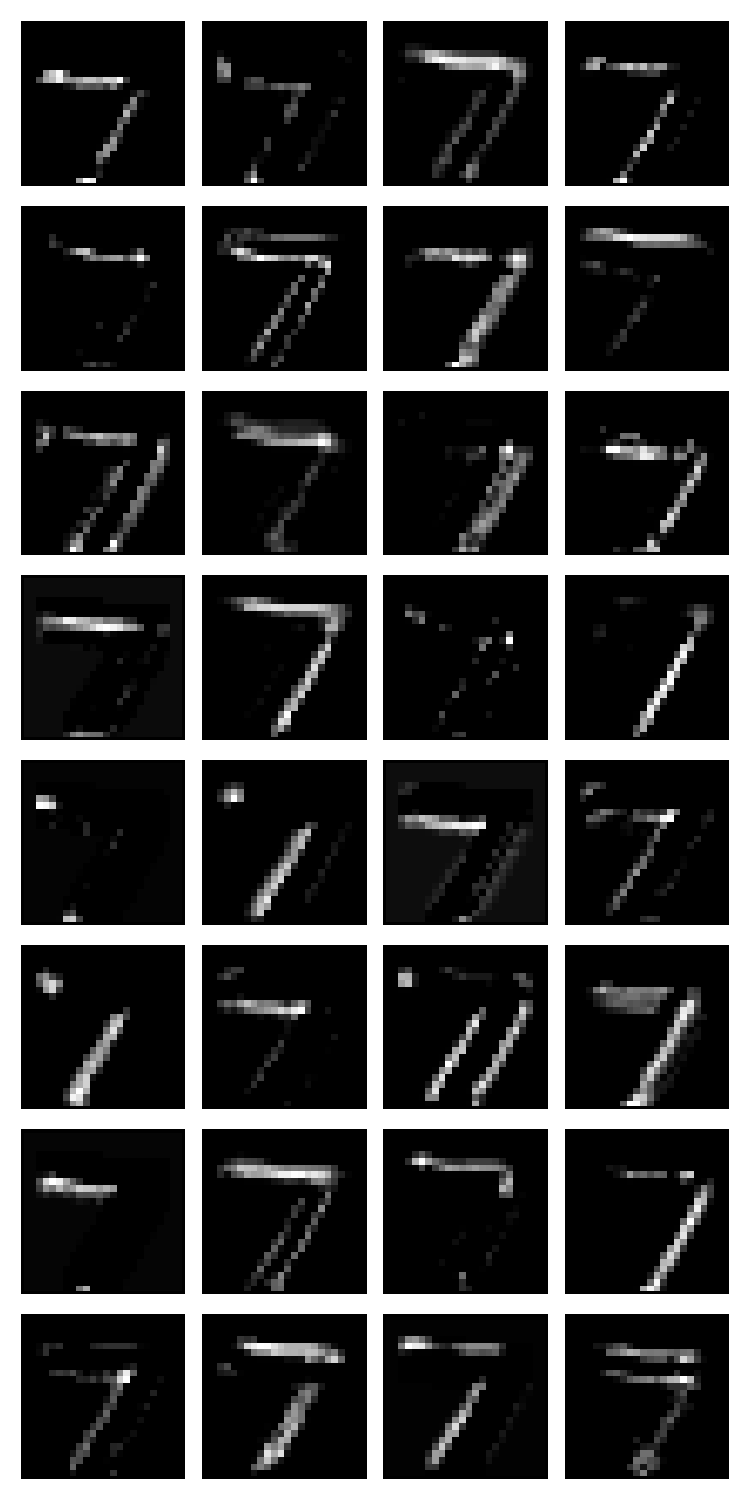
\includegraphics[width=\textwidth]{keras_l1_outputs.pdf}
\column{0.2\textwidth}
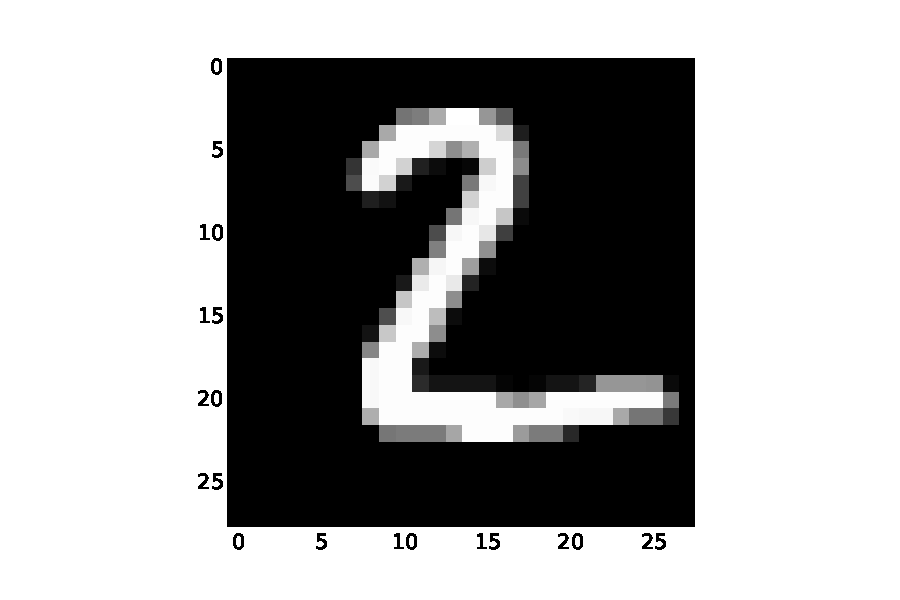
\includegraphics[width=\textwidth]{keras_l1_input_2.pdf}\\
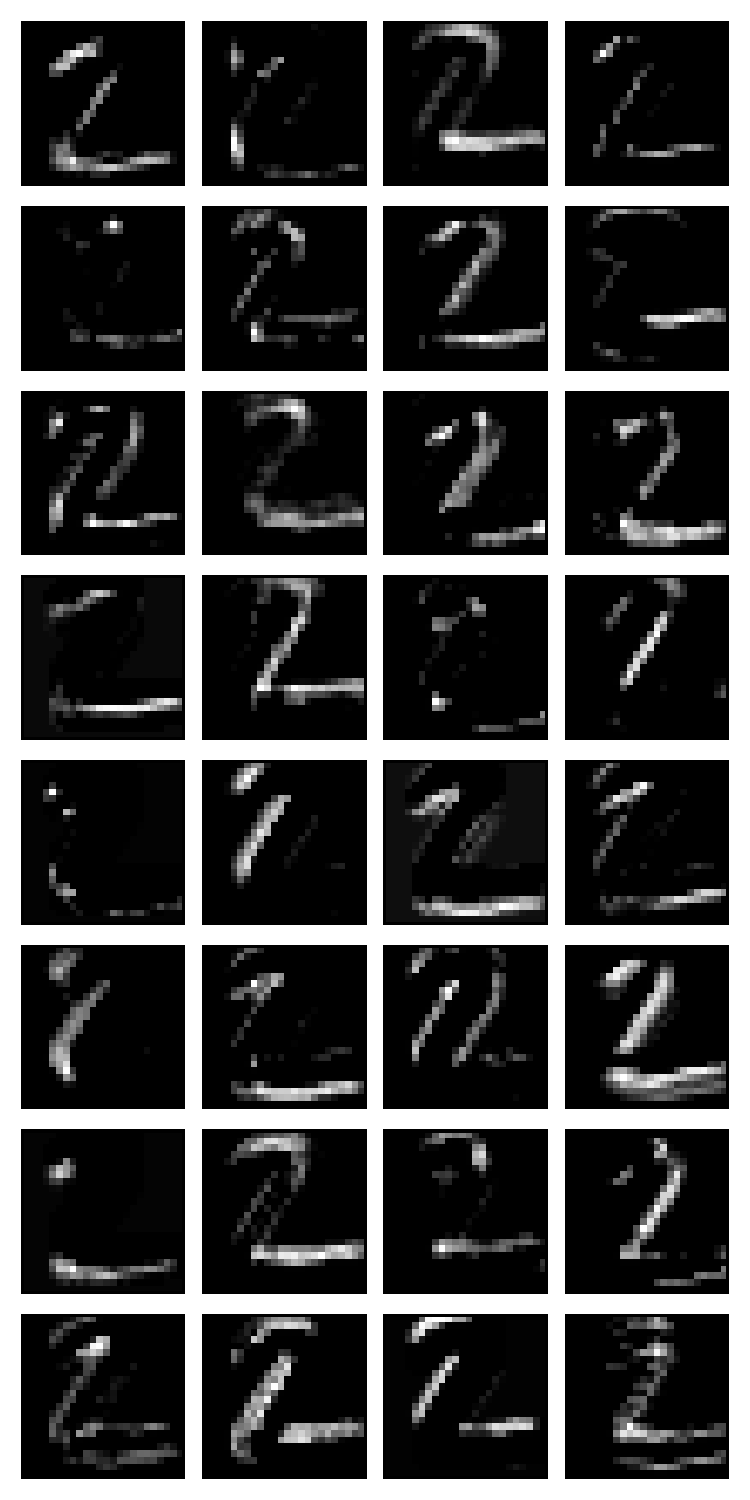
\includegraphics[width=\textwidth]{keras_l1_outputs_2.pdf}
\end{columns}
\end{frame}

\begin{frame}[fragile]{Second Layer Activations}
\begin{columns}
\column{0.6\textwidth}
\begin{itemize}
	\item On the next layer, the figures are downsampled to 12x12.
	\item This provides \emph{spatial invariance}: The same activation results although the input would be slightly displaced.
	\end{itemize}
\column{0.2\textwidth}
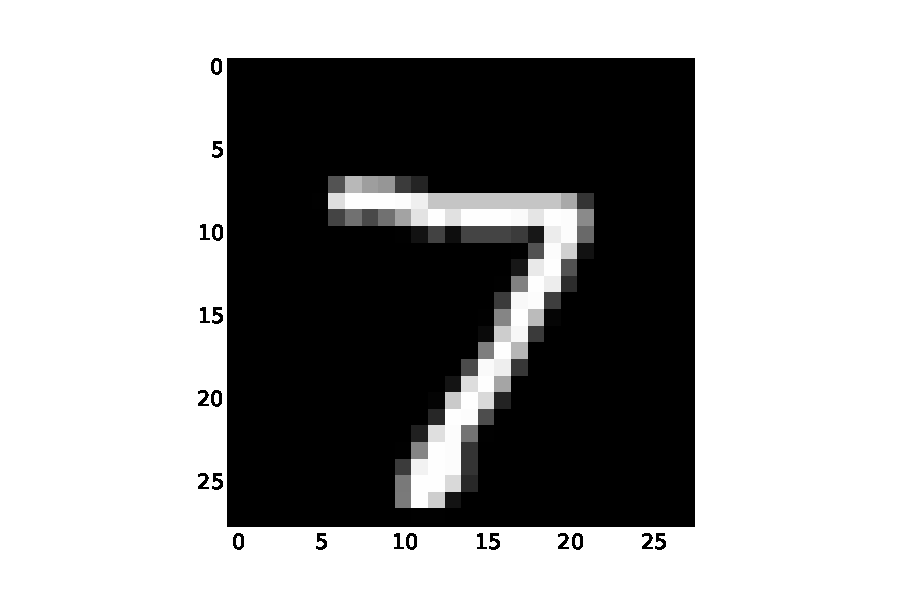
\includegraphics[width=\textwidth]{keras_l1_input.pdf}\\
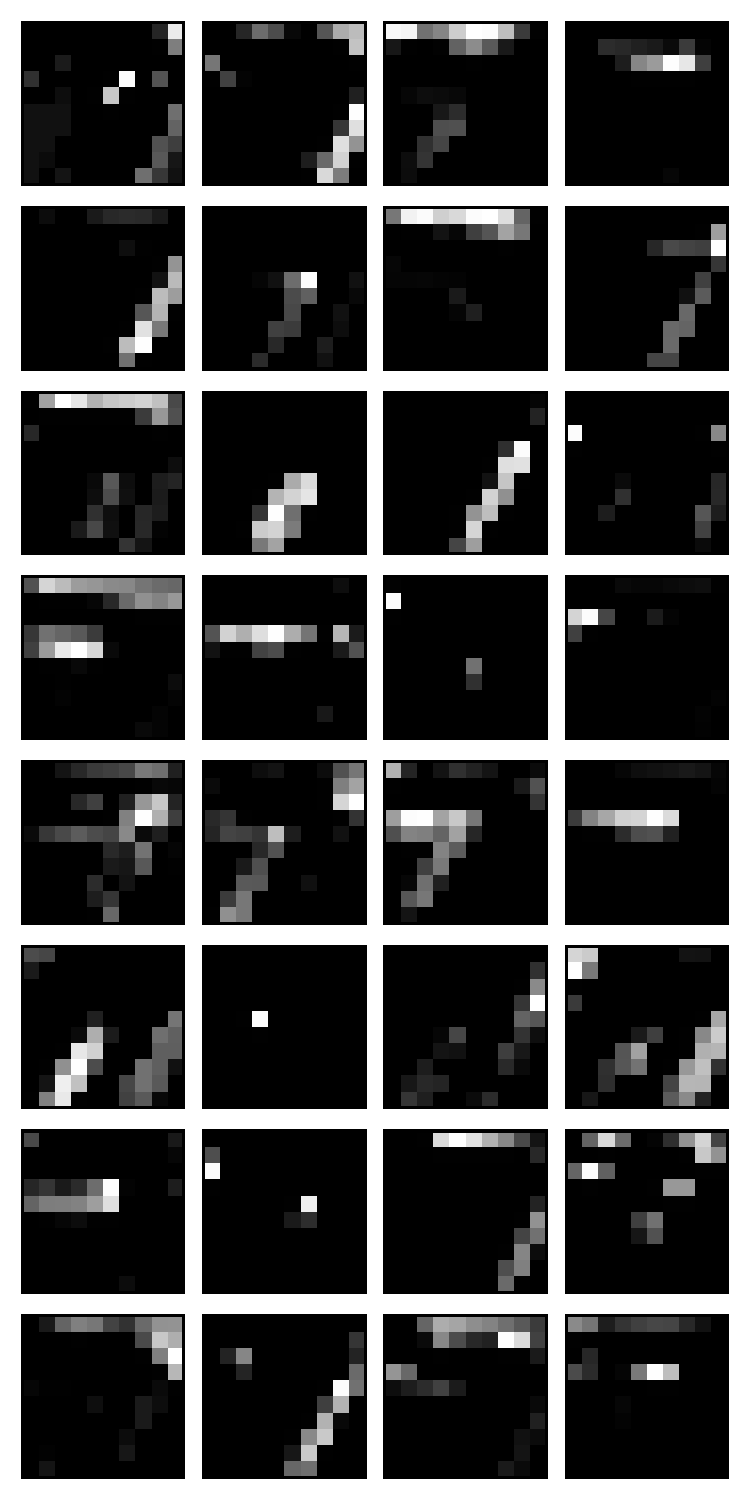
\includegraphics[width=\textwidth]{keras_l2_outputs.pdf}
\column{0.2\textwidth}
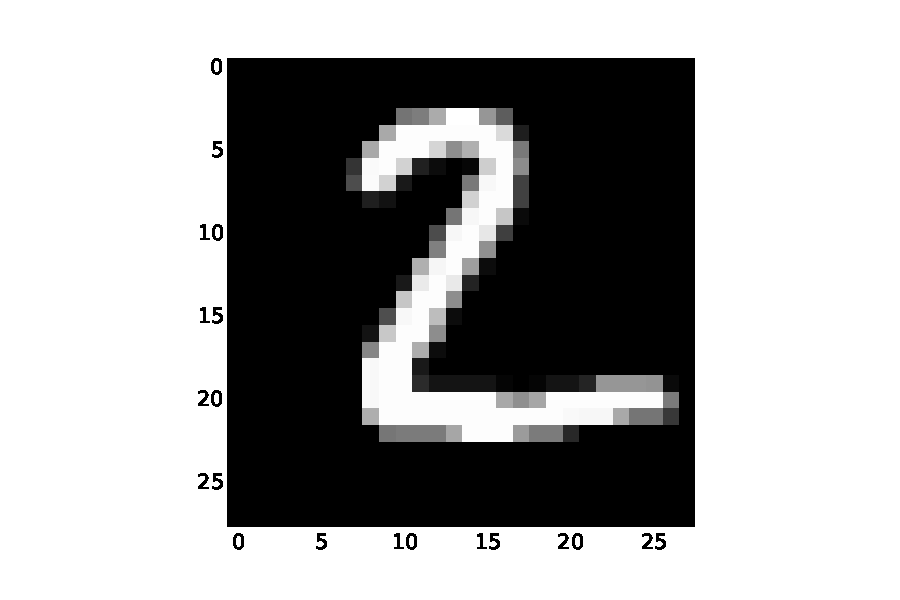
\includegraphics[width=\textwidth]{keras_l1_input_2.pdf}\\
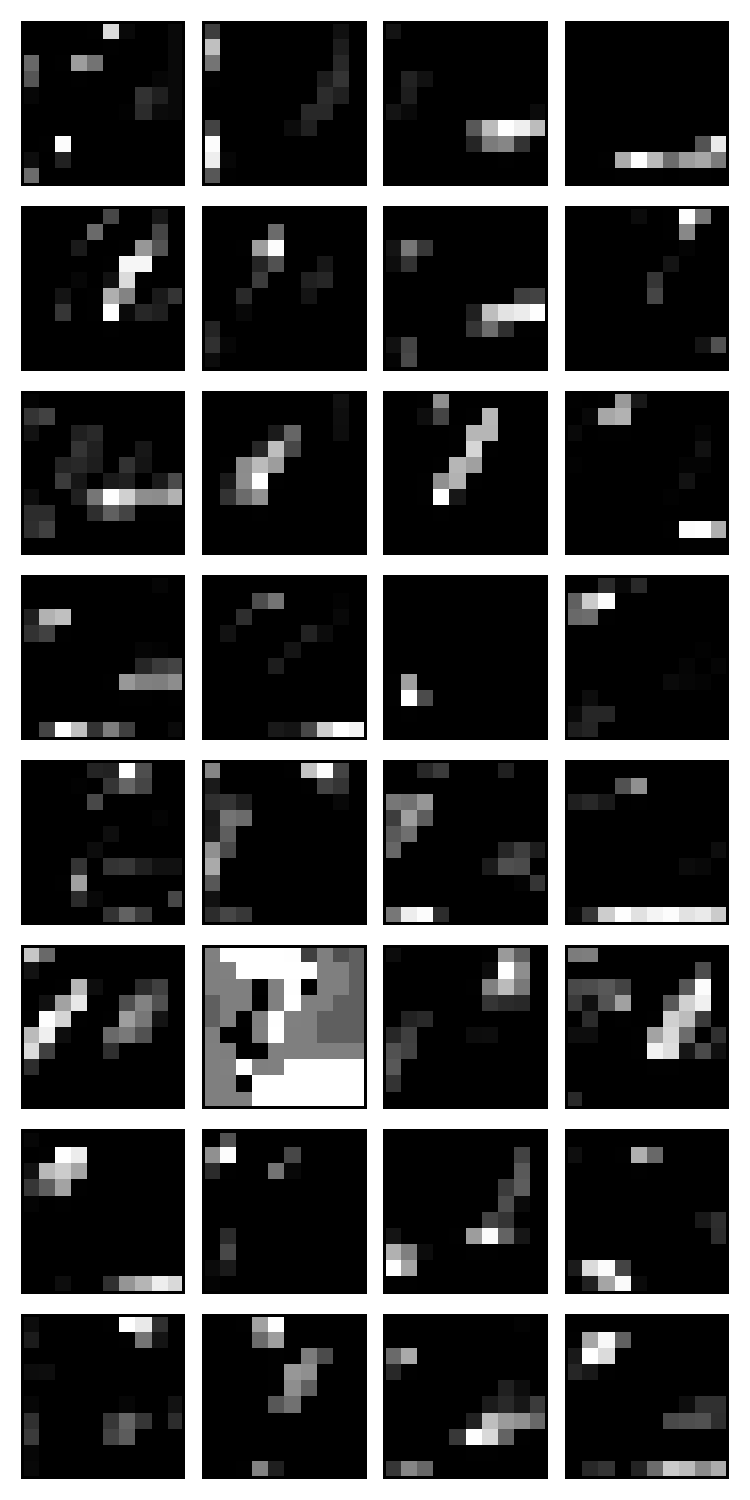
\includegraphics[width=\textwidth]{keras_l2_outputs_2.pdf}
\end{columns}
\end{frame}



\end{document}

